\documentclass[a4paper]{article}

\usepackage{color}
\usepackage{url}
\usepackage[T2A]{fontenc} % enable Cyrillic fonts
\usepackage[utf8]{inputenc} % make weird characters work
\usepackage{graphicx}

\usepackage[english,serbian]{babel}
%\usepackage[english,serbianc]{babel} %ukljuciti babel sa ovim opcijama, umesto gornjim, ukoliko se koristi cirilica

\usepackage[unicode]{hyperref}
\hypersetup{colorlinks,citecolor=green,filecolor=green,linkcolor=blue,urlcolor=blue}

%\newtheorem{primer}{Пример}[section] %ćirilični primer
\newtheorem{primer}{Primer}[section]

	\title{Reklame na društvenim mrežama\\ \small{Seminarski rad u okviru kursa\\Tehničko i naučno pisanje\\ Matematički fakultet}}
	
	\author{Natalija Pavlićević (pavlicevicnatalija@gmail.com)\\ Teodora Maksimović (teamax18@gmail.com)\\ Branka Marković (bakymarkovic@gmail.com)\\ Mihailo Damnjanović (mihailo.damnjanović@gmail.com)}
	\date{15.~novembar 2022.}
	\maketitle
	
	\abstract{Ovo je apstrakt za ovaj seminarski rad.
	}

\tableofcontents

\newpage

\begin{document}
	
	\section{Prikupljanje podataka korisnika}
	\label{sec:podaci}
	Oglašivači sve više koriste personalizovano reklamiranje koje je prilagođeno potrošačima na osnovu podataka koji se tiču njihovih preferencija i ponašanja, a koje dobijaju prikupljanjem njihovih ličnih podataka. Ciljano reklamiranje je sve veća oblast interesovanja za i poslovne i istraživačke zajednice. Reklame u mobilnim uslugama i oglasi u aplikaciji predstavljaju oblast rasta u nastajanju, u kojoj ciljano reklamiranje postaje sve važniji izvor prihoda i za oglašivače i za reklamne kompanije. Ciljano reklamiranje se zasniva na analitici velikih podataka, gde lični podaci korisnika se prikupljaju i obrađuju za svrhe profilisanja i ciljanja.
	

	\section{Misljenje korisnika o reklamama na internetu}
	\label{sec:misljenje}
	Kroz istrazivanje o misljenju korisnika za reklame na internetu, dosli smo do zakljucka da se misljenja razlikuju i da ima korisnika kojima smetaju reklame, a ima i onih koji vole da kliknu i vide sta im se ponudi u reklami.
	Same reklame korisnicima mogu da smetaju prilikom koriscenja nekih aplikacija ili gledanja filmova,kao i na youtube-u dok slusaju muziku jer reklame samo iskacu.To korisnicima kvari dogadjaj i oni samo preskacu te reklame.
	Medjutim, naravno da ima korisnika i koji vole kad im iskoci neka reklama, narocito ako se oni u tom trenutku tragaju za tim proizvodima koji se reklamiraju, oni klikcu na reklame.
	\subsection{Da li korisnici veruju reklamama na internetu?}
	\label{subsec:veovanje_reklamama}
	Dosta korisnika veruje reklamama na internetu ali samo onim koji su provereni ili se pronalaze u njima.Naravno ima odredjeni broj korisnika koji ne veruje reklamama i oni misle da su te reklame samo prevare koje privlace korisnike da kupe proizvode koji nisu tako dobri kao na reklama.U nastavku mozete videti sliku \ref{fig:verovanje_reklamama} koliko procenata veruje,a koliko ne.
	\begin{verbatim}
		\usepackage{graphicx}
	\end{verbatim}
	
	\begin{figure}[h!]
		\begin{center}
			\includegraphics[scale=0.75]{verovanje_reklamama.jpg}
		\end{center}
		\caption{verovanje_reklamama}
		\label{fig:verovanje_reklamama}
	\end{figure}
	Ovo istrazivanje izvrseno je od strane Social Serbia 2020.
	\subsection{Koliko cesto korisnici klikcu na reklame?}
	\label{subsec:klik_na_reklamu}
	Zanimljiva cinjenica kod ovoga jeste to da je veci procenat muskaraca koji cesto klikcu na reklame nego zena. u nastavku mozete videti sliku \ref{fig:klik_na_reklamu} koliko cesto korisnici klikcu na reklame.
		\begin{verbatim}
		\usepackage{graphicx}
	\end{verbatim}
	
	\begin{figure}[h!]
		\begin{center}
			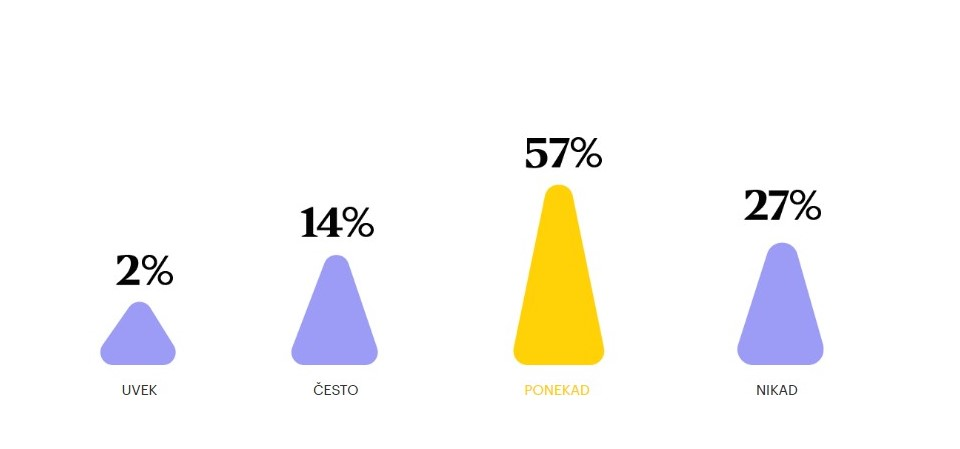
\includegraphics[scale=0.75]{klik_na_reklamu.jpg}
		\end{center}
		\caption{klik_na_reklamu}
		\label{fig:klik_na_reklamu}
	\end{figure}
	Takodje i ovo istrazivanje izvrseno je od strane Social Serbia 2022.
	\section{Doprinos od reklama}
	\label{sec:doprinos}
	\subsection{Da li se treba reklamirati?}
	\label{subsec:potrebna_reklama}
	
\end{document}